\begin{center}
    \section*{\huge{序 \quad 言}}
\end{center}

\vspace{1cm}

\thispagestyle{empty}

\doublespacing

苦于没有完整的电动力学真题集与解析，这给备考院大电动力学带来了诸多不便，因而笔者整理了本文档并给出了一些题目的解析。本文档包含了中国科学院大学2006年电动力学A卷，B卷，2007年电动力学A卷，B卷，2008年电动力学，2009年电动力学，2011年电动力学回忆版，2012年电动力学，2013年电动力学，2014年电动力学，2015年电动力学，2016年电动力学，2017年电动力学，2020年电动力学，2021年电动力学，2023年电动力学回忆版，及2024年电动力学回忆版与部分题目的解析。虽有部分年份没有真题甚至没有回忆版的真题，但是对于备考电动力学专业课，结合本文档真题与郭书已经足够。

由于笔者水平有限，该文档可能会有一些错误，包括但不限于：错别字，用词错误，句子表达问题，公式的错误，字形的问题，标点符号的错误，版面的问题，排版的问题等。

在编写本文档的过程中参考了\url{https://gitee.com/ylxdxx/AM601-kaoyan}的 \LaTeX 源码，在学习电动力学的过程中，下方QQ群群友给予了我不少帮助，特在此表示感谢。也欢迎需要备考电动力学的同学加入该群，如果该文档有任何问题，欢迎补充！

\LaTeX 源码地址：\url{\url{https://www.overleaf.com/read/ynyhjbzkqxcz#780638}}。如果需要对本文档进行修改，可以通过overleaf 在线编辑，Readme文件夹中包含对该文档编辑的说明。


% 本文档\LaTeX 代码源码地址：\\


\begin{center}
	\kaishu 
        \Large{“愿君莫负韶华，祝君金榜题名!”}
\end{center}

% \vspace{0.5cm}

\begin{center}
	\flushright
	\begin{tabular}{c}
		xc  \\
		\today
	\end{tabular}	
\end{center}

\begin{figure}[h]
    \centering
    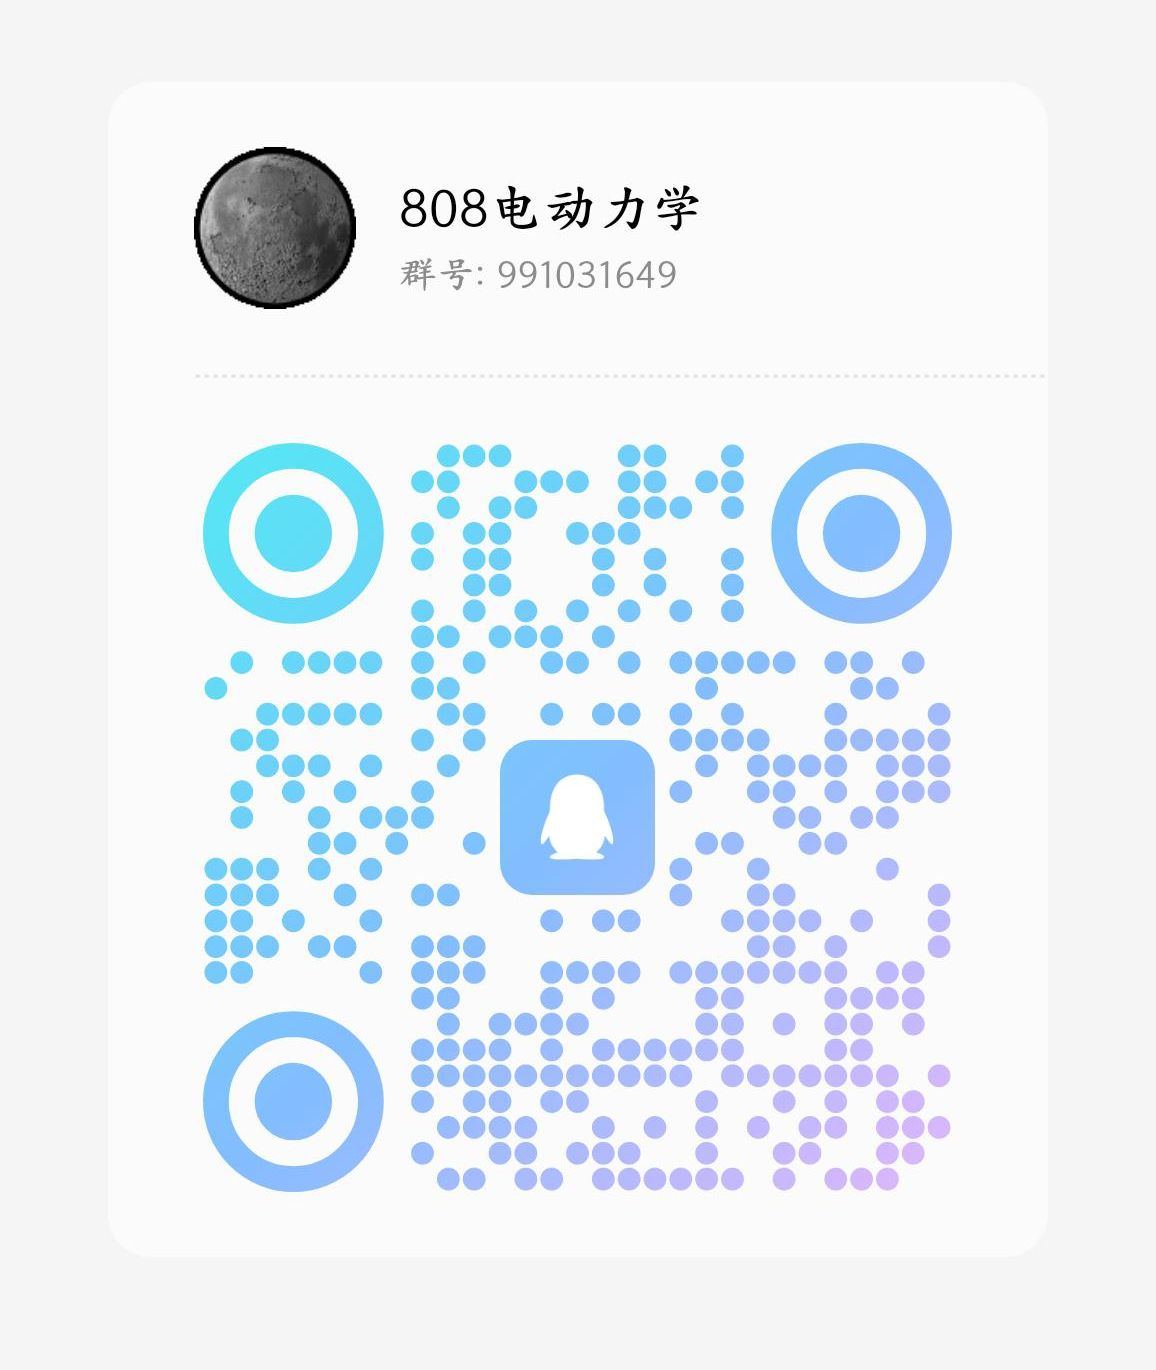
\includegraphics[width=0.35\linewidth]{808/QQ.jpg}
        \label{fig:QQ}
        \end{figure}

\clearpage
\phantom{s}
\clearpage